\RequirePackage[l2tabu, orthodox]{nag}
\documentclass{article}

\newcounter{chapter}
\setcounter{chapter}{6} % Modify Counter To Chapter

\setcounter{section}{\value{chapter}}
\addtocounter{section}{-1}

\usepackage{amssymb,amsmath,verbatim,graphicx,microtype,units,booktabs}
\usepackage[margin=10pt, font=small, labelfont=bf, labelsep=endash]{caption}
\usepackage[colorlinks=true, pdfborder={0 0 0}]{hyperref}
\usepackage[utf8]{inputenc}
\usepackage{pdfpages}

\usepackage[left=0.75in, right=0.75in]{geometry}
\usepackage{titleps}
\newpagestyle{main}{
    \setheadrule{.4pt}
    \sethead{Chapter \thechapter: \sectiontitle}
            {}
            {Illya Starikov}
}
\pagestyle{main}

\begin{document}
\section{Learning}

\subsection{Class Notes}
\begin{itemize}
    \item Neutral stimulus = no response
    \item Unconditioned stimulus = unconditioned response
    \item Pavlov = dogs, watson = people, skinner = operant conditioning (reward / punish), Bandura = observation
\end{itemize}

\subsection{Study Guide Material}
\begin{description}
    \item [Aversive conditioning] is an aspect of operant conditioning that deals with unpleasant stimuli and how we learn to stay away from them.
    Escape is defined as performing an operant response to cause an aversive stimulus to cease (ex. run to the other side of a shuttle box to get away from shock).
    \item [Observational] learning occurs when an organism’s response is influenced by the observation of others, who are called models.
    \item [Positive] reinforcement occurs when a response is strengthened because it is followed by the presentation of a rewarding stimulus.
    \item [Responses] can be strengthened either by presenting positive reinforcers or by removing negative reinforcers.
    \item [John Watson] is referred to as the ‘father of modern behaviorism’ and was influenced by Pavlov’s work.
    Classical conditioning can be broken down into two basic parts – acquisition and extinction.  Acquisition is the initial stage of learning something – like Pavlov’s dog learning to drool at the tone of the bell. The graph here shows the strength of the dog’s response, measured in \item drops of saliva, to the conditioned stimulus (the bell).
    \item [Extinction] is the process by which the association between the unconditioned stimulus (meat powder) and conditioned stimulus (bell ringing) is broken.
    \item [Spontaneous recovery] is an extinguished conditioned stimulus suddenly elicits a conditioned response again.
    \item [Aversive conditioning] is an aspect of operant conditioning that deals with unpleasant stimuli and how we learn to stay away from them.
    \item [Intermittent reinforcement], or partial reinforcement, occurs when a designated response is reinforced only some of the time.
    \item [Unconditioned stimulus] no stimulus without conditioning (US). Conditioned response  a learned reaction from previous conditioning (CR).
    \item [Acquisition] is the initial stage of learning a new response.
    Skinner’s principle of reinforcement holds that organisms tend to repeat those responses that are followed by favorable consequences, or reinforcement. Something is positively reinforcing if individuals are reinforced when it is presented to them, like food, water, sleep, or sex.
    \item [Operant conditioning] is a form of learning in which responses come to be controlled by their consequences.
\end{description}

\subsection{Book Notes}
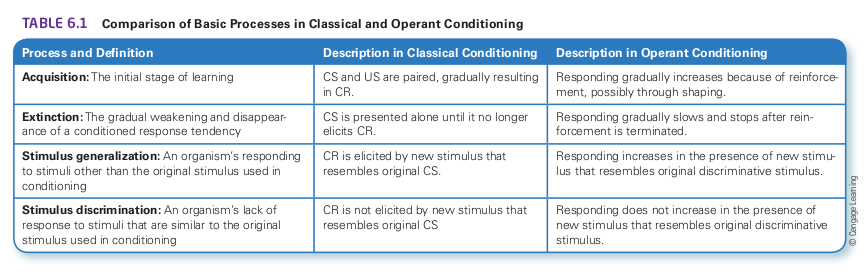
\includegraphics[width=\textwidth]{process}
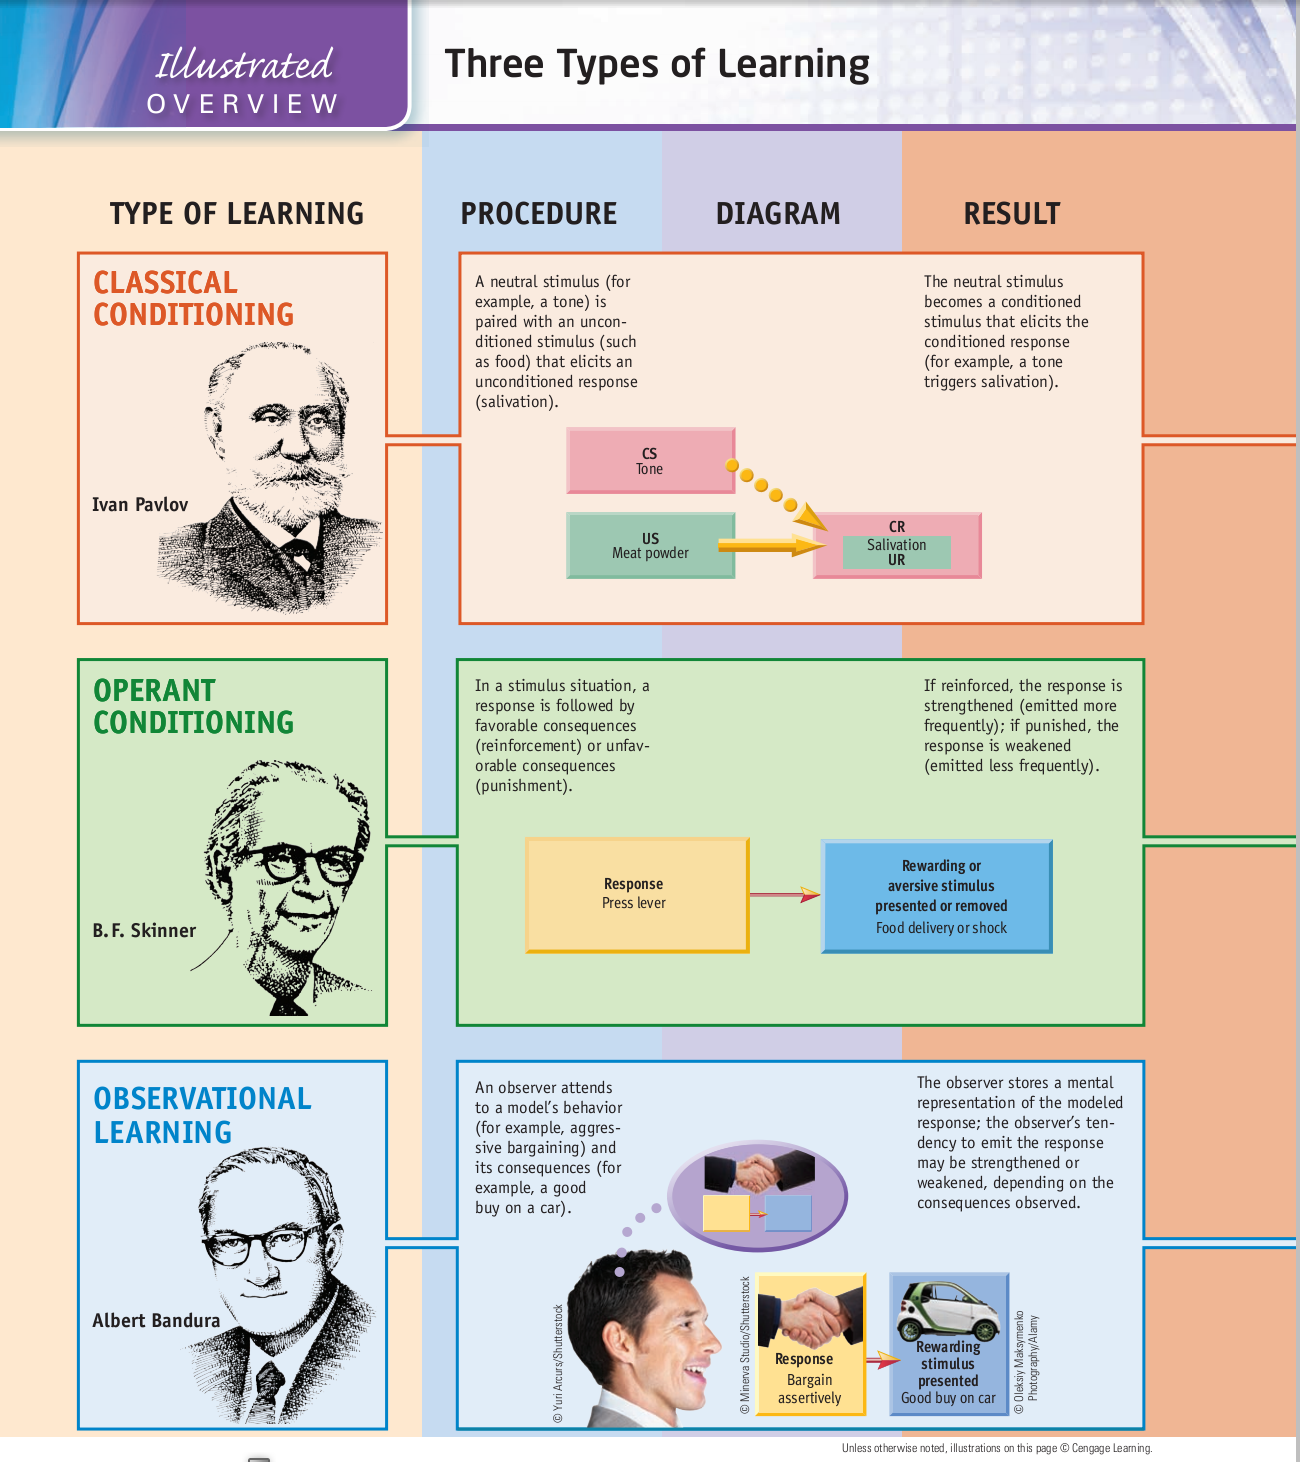
\includegraphics[width=\textwidth]{types}
\end{document}